\documentclass[10pt,aspectratio=169]{beamer}
\usetheme{metropolis}
\usepackage{appendixnumberbeamer}
\usepackage{booktabs}
\usepackage{graphicx}
\usepackage{tikz}
\usepackage{amsmath}
\usepackage{xcolor}

% Define NHS colors
\definecolor{nhsblue}{RGB}{0,94,184}
\definecolor{nhsdarkblue}{RGB}{0,48,135}
\definecolor{nhsgreen}{RGB}{0,177,64}
\definecolor{nhsred}{RGB}{218,41,28}

% Set theme colors
\setbeamercolor{frametitle}{bg=nhsblue,fg=white}
\setbeamercolor{progress bar}{fg=nhsgreen}
\setbeamercolor{title separator}{fg=nhsblue}
\setbeamercolor{alerted text}{fg=nhsred}

\metroset{progressbar=frametitle,sectionpage=progressbar,numbering=fraction}

% Command for watermark apes as background
\newcommand{\apewatermark}[1]{%
    \setbeamertemplate{background}{%
        \begin{tikzpicture}[remember picture,overlay]
            \node[anchor=south east,inner sep=1cm] at (current page.south east) {
                \includegraphics[height=3cm]{#1}
            };
        \end{tikzpicture}
    }
}

\title{AMD Protocol Explorer (APE)}
\subtitle{Agent-Based Simulation for Neovascular AMD Treatment Planning}
\author{Luke Herbert\\Consultant Ophthalmologist}
\institute{Surrey and Sussex Healthcare NHS Trust}
\date{24th June 2025}

\begin{document}

% Customize title page to add banana ape
{
\setbeamertemplate{title page}{
  \begin{minipage}[b][\paperheight]{\textwidth}
    \vfill
    \ifx\inserttitlegraphic\@empty\else\usebeamertemplate*{title graphic}\fi
    \vfill
    \ifx\inserttitle\@empty\else\usebeamertemplate*{title}\fi
    \ifx\insertsubtitle\@empty\else\usebeamertemplate*{subtitle}\fi
    \usebeamertemplate*{title separator}
    \ifx\insertauthor\@empty\else\usebeamertemplate*{author}\fi
    \ifx\insertdate\@empty\else\usebeamertemplate*{date}\fi
    \ifx\insertinstitute\@empty\else\usebeamertemplate*{institute}\fi
    \vfill
    \centering
    
\includegraphics[height=2.5cm]{banana_ape.png}
    \vspace{0.5cm}
  \end{minipage}
}
\maketitle
}

% Acknowledgments in title frame note
\begin{frame}{Acknowledgments}
\begin{itemize}
    \item Health Service Modelling Associates (HSMA) team
    \item Finance Director and IT Director
    \item NHS England Pharmacy \& Clinical Support Team
\end{itemize}
\end{frame}

\section{Understanding Neovascular AMD}

\begin{frame}{What is Neovascular AMD (NAMD)?}
\begin{columns}[T]
\column{0.5\textwidth}
\begin{itemize}
    \item Leading cause of central vision loss
    \item Cannot read or recognize faces
    \item Leads to legal blindness if untreated
    \item Affects quality of life severely
\end{itemize}

\column{0.5\textwidth}
\begin{figure}
    \centering
    
\includegraphics[width=0.8\textwidth]{logMAR_chart_explainer.png}
\end{figure}
\end{columns}

\vspace{0.5cm}
\begin{columns}[T]
\column{0.5\textwidth}
\begin{figure}
    \centering
    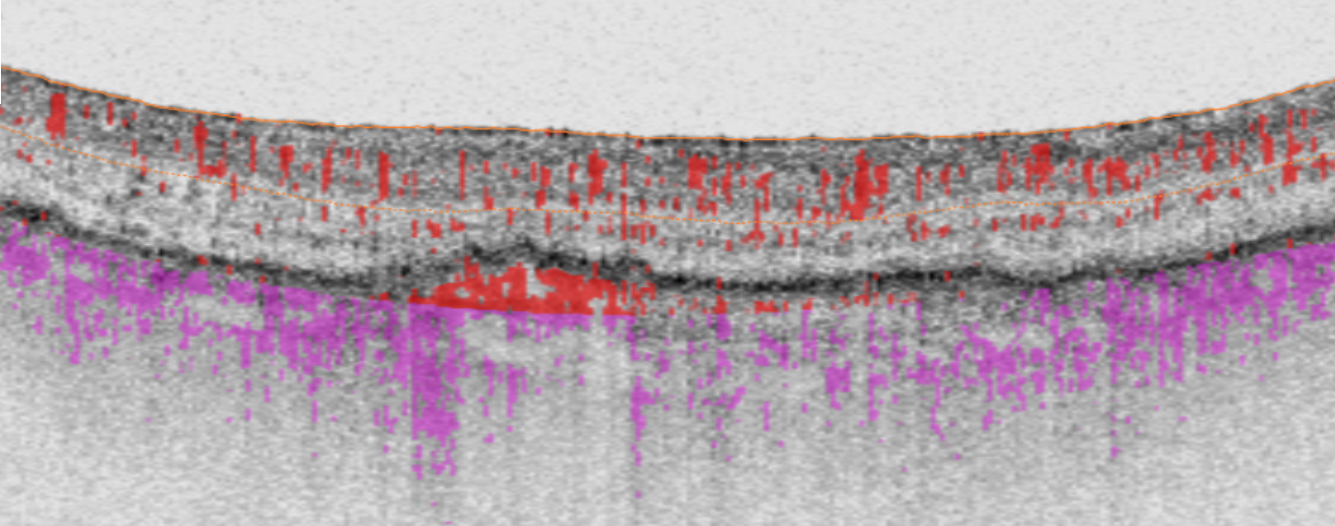
\includegraphics[width=0.9\textwidth]{early-namd-b-scan.png}
\end{figure}

\column{0.5\textwidth}
\begin{figure}
    \centering
    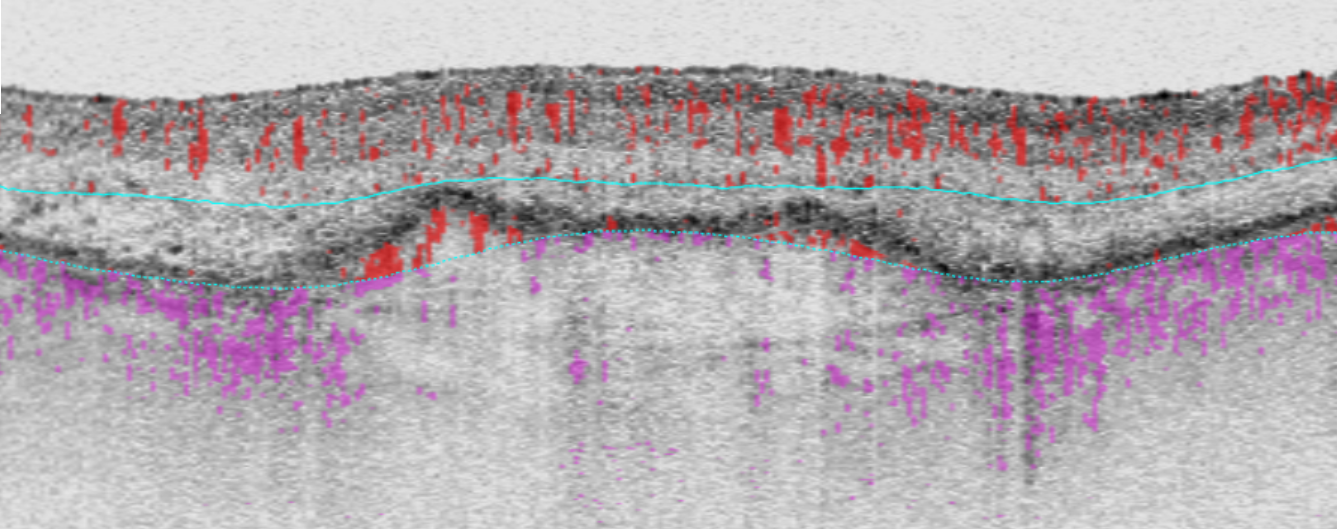
\includegraphics[width=0.9\textwidth]{later-namd-b-scan.png}
\end{figure}
\end{columns}
\end{frame}

\begin{frame}{The Biology Behind NAMD}
\begin{columns}[T]
\column{0.6\textwidth}
\textbf{Disease Process:}
\begin{itemize}
    \item Aging eye environment
    \item Increased VEGF (Vascular Endothelial Growth Factor)
    \item Abnormal blood vessel growth
    \item Leakage, fibrosis, and bleeding
\end{itemize}

\column{0.4\textwidth}
\begin{exampleblock}{VEGF?}

  VEGF is like fertiliser for blood vessels. Anti-VEGF is something that removes the fertiliser.

  As VEGF keeps being made we have to keep removing it.
  \end{exampleblock}
\end{columns}
\end{frame}

{
\setbeamertemplate{section page}{
  \centering
  \vspace{2cm}
  {\usebeamerfont{section title}\usebeamercolor[fg]{section title}\insertsection}\\
  \vspace{1cm}
  
\includegraphics[height=4cm]{hope_ape.png}
}
\section{Hope}
}

\begin{frame}{Revolutionary Treatment: Anti-VEGF Therapy}
\begin{columns}[T]
\column{0.6\textwidth}
\textbf{How it works:}
\begin{itemize}
    \item Antibodies or similar molecules bind to VEGF
    \item Remove growth factor from eye
    \item Stop abnormal vessel growth
\end{itemize}

\vspace{0.5cm}
\alert{\textbf{The Challenge:}}
\begin{itemize}
    \item Molecules cleared over time
    \item Requires repeated injections
    \item Optimal frequency unknown
\end{itemize}

\column{0.4\textwidth}
\begin{figure}
    \centering
    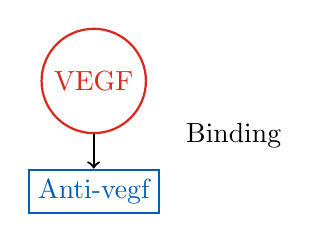
\begin{tikzpicture}[scale=0.7]
        % VEGF binding diagram
        \node[circle,draw,nhsred,thick,minimum size=1cm] (vegf) at (0,2) {VEGF};
        \node[draw,nhsblue,thick,minimum width=1.5cm] (ab) at (0,0) {Anti-vegf};
        \draw[->,thick] (vegf) -- (ab);
        \node[right] at (1.5,1) {Binding};
    \end{tikzpicture}
\end{figure}
\end{columns}
\end{frame}

\begin{frame}{Real-World Treatment Challenges}
\begin{alertblock}{Why Patients Stop Treatment}
\begin{itemize}
    \item \textbf{Mortality}: Elderly population (average age 80+)
    \item \textbf{Frailty}: Too unwell to attend monthly appointments
    \item \textbf{Treatment failure}: Vision deteriorates despite therapy
    \item \textbf{NHS capacity}: Limited appointment availability
\end{itemize}
\end{alertblock}

\begin{block}{Discontinuation Rates}
\begin{itemize}
    \item Year 1: 10-15\% stop treatment
    \item Year 2: Additional 10-15\%
    \item By Year 5: Only 50-60\% still on treatment
\end{itemize}
\end{block}

\end{frame}

{
\setbeamertemplate{section page}{
  \centering
  \vspace{2cm}
  {\usebeamerfont{section title}\usebeamercolor[fg]{section title}\insertsection}\\
  \vspace{1cm}
  
\includegraphics[height=4cm]{sad_ape_watermark.png}
}
\section{The Cost Challenge}
}

\begin{frame}{NHS Annual Treatment Costs}
\apewatermark{sad_ape_watermark.png}
\begin{table}
\centering
\begin{tabular}{lrr}
\toprule
Treatment Area & Annual NHS Spend & Annual Patient Numbers \\
\midrule
\alert{Wet AMD (Anti-VEGF)} & \alert{£600-800 million} & 40,000 new, ~200,000 continuing \\
Cataract Surgery & £320-480 million & 400,000 \\
Hip Replacement & £500-700 million & 100,000 \\
\bottomrule
\end{tabular}
\end{table}

\vspace{0.3cm}
\begin{alertblock}{Cost per QALY}
\begin{itemize}
    \item Cataract surgery: £1,964 per QALY (exceptional value)
    \item Hip replacement: £2,128 per QALY (strong value)
    \item \alert{Wet AMD: £58,047 per QALY (3x NICE threshold)}
\end{itemize}
\end{alertblock}

\begin{block}{Current Anti-VEGF Drug Costs (2024 list prices)}
\begin{itemize}
    \item Aflibercept (Eylea): £816 a dose, generic soon maybe £400
    \item Patients need 7-10 injections year 1, then 4-6/year ongoing
\end{itemize}
\end{block}

\centering
\textbf{Challenge: £1.2-1.5 billion projected cost by 2035}
\end{frame}

% Clear the background for subsequent frames
\setbeamertemplate{background}{}

{
\setbeamertemplate{section page}{
  \centering
  \vspace{2cm}
  {\usebeamerfont{section title}\usebeamercolor[fg]{section title}\insertsection}\\
  \vspace{1cm}
  
\includegraphics[height=4cm]{thoughtful_ape.png}
}
\section{Why Model?}
}

\begin{frame}{The Need for Modeling}
\begin{columns}[T]
\column{0.5\textwidth}
\textbf{Current Challenges:}
\begin{itemize}
    \item Complicated and tangled evidence base
    \item Limited real-world data
    \item Complex patient pathways
    \item Resource constraints
\end{itemize}

\column{0.5\textwidth}
\textbf{Modeling Benefits:}
\begin{itemize}
    \item Promote discussion
    \item Clarify outcome measures
    \item Explore treatment strategies
    \item Evidence-based decisions
    \item Predict resource needs
    \item Balance drug versus other costs
\end{itemize}
\end{columns}
\end{frame}

\begin{frame}{Two Modeling Approaches}
\begin{columns}[T]
\column{0.5\textwidth}
\textbf{Simple Approach (NHS England):}
\begin{itemize}
    \item Excel spreadsheet
    \item "Best guess" parameters
    \item Average patient behavior
    \item Quick but limited insights
\end{itemize}

\column{0.5\textwidth}
\textbf{Our Approach (Agent-Based):}
\begin{itemize}
    \item Individual patient simulation
    \item Build from known parameters
    \item Probabilistic events
    \item Rich, detailed insights
\end{itemize}
\end{columns}

\vspace{0.5cm}
\centering

\begin{tikzpicture}
    \node[draw,nhsblue,thick,minimum width=3cm] (excel) at (0,0) {Excel Model};
    \node[draw,nhsgreen,thick,minimum width=3cm] (agent) at (7,0) {Agent-Based Model};
    \draw[->,thick] (excel.east) -- node[above] {Evolution} (agent.west);
\end{tikzpicture}
\end{frame}

\begin{frame}{Real-World Complexity in Our Simulation}
\begin{alertblock}{}
\begin{columns}[T]
\column{0.5\textwidth}
\textbf{Simple Models Assume:}
\begin{itemize}
    \item All patients start with same vision
    \item Perfect treatment adherence
    \item No appointment delays
    \item Uniform response to treatment
\end{itemize}

\column{0.5\textwidth}
\textbf{Our Simulation Includes:}
\begin{itemize}
    \item Vision distribution at baseline
    \item Real discontinuation patterns
    \item Treatment gaps and delays
    \item Individual patient trajectories
\end{itemize}
\end{columns}
\end{alertblock}

\vspace{0.5cm}
\begin{center}
\begin{minipage}{0.7\textwidth}
\begin{block}{Why This Matters}
\begin{itemize}
    \item Captures NHS capacity constraints
    \item Models actual patient populations
    \item Predicts realistic outcomes
    \item Enables better resource planning
\end{itemize}
\end{block}
\end{minipage}
\end{center}
\end{frame}

\section{The APE}

\begin{frame}{Application Architecture}
\centering
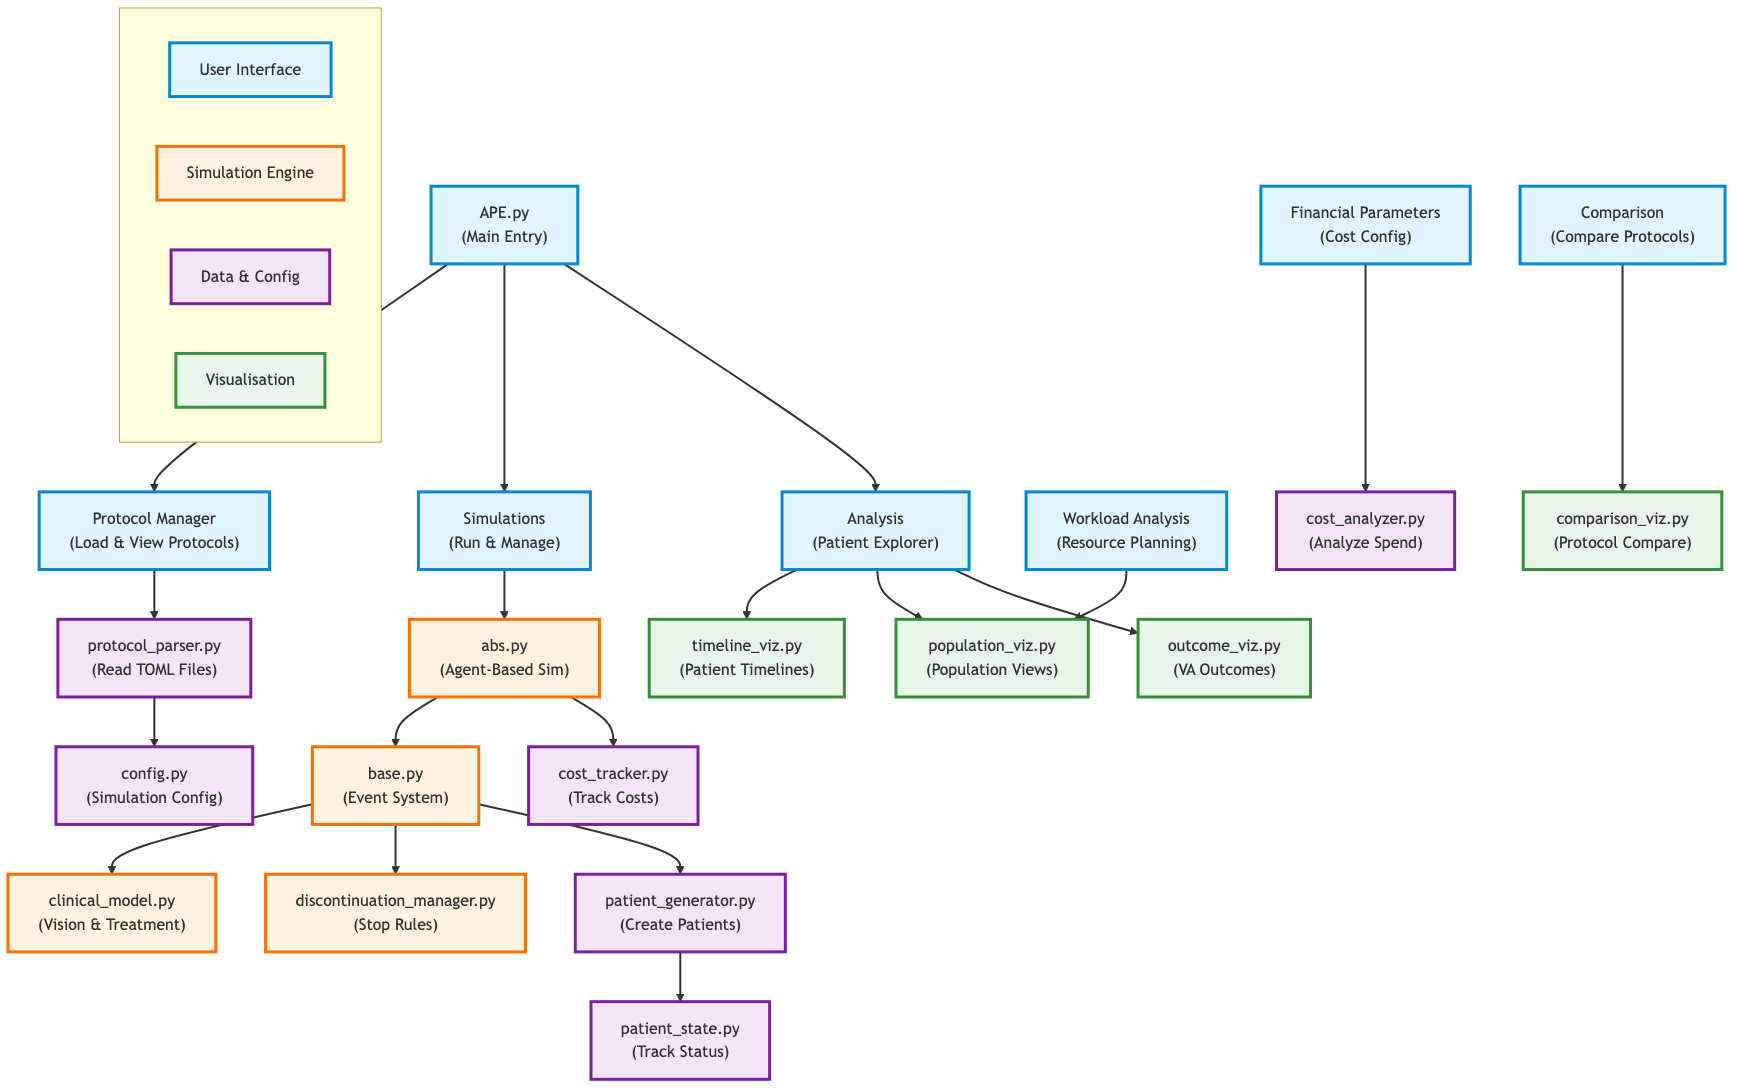
\includegraphics[width=\textwidth,height=0.85\textheight,keepaspectratio]{ape_architecture.png}
\end{frame}

% Placeholder for screen recording section
\begin{frame}{Demonstration}
\end{frame}

\section{Thoughts}

\begin{frame}{What We've Learned}
\begin{columns}[T]
\column{0.5\textwidth}
\textbf{Model Reveals:}
\begin{itemize}
    \item Treatment pattern impacts
    \item Resource utilization peaks
    \item Patient outcome distributions
    \item Protocol efficiency metrics
\end{itemize}

\column{0.5\textwidth}
\textbf{Enables:}
\begin{itemize}
    \item Evidence-based protocols
    \item Capacity planning
    \item Cost-effectiveness analysis
    \item Commissioning decisions
\end{itemize}
\end{columns}

\vspace{0.5cm}
\begin{alertblock}{New Feature}
Cost calculator module now available for full economic analysis
\end{alertblock}
\end{frame}

\begin{frame}{Thank You}
\centering
\Large
Questions?

\vspace{1cm}
\normalsize
\textbf{Contact:}\\
l.herbert@nhs.net

\vspace{0.5cm}
\textbf{Project Repository:}\\
\url{https://github.com/lh/vegf-1} \\
\textbf{Application:}\\
\url{https://vegf-1.streamlit.app}

\vspace{0.5cm}
\textbf{Acknowledgments:}\\
HSMA Team | NHS England | Trust Leadership
\end{frame}

\end{document}